\chapter{Issues and Future Work}


\section{Issues} 
One of the design issues faced during the development is where should the SDK be installed from Architecture point of view?
1-On the server side where the hyperledger fabric lives?  or 2-On the client side (Android side) taking into consideration there is no official support for an Android SDK. The only supported SDKs are on GO, javascript, and java.
Building and integrating an Android SDK from scratch is nontrivial it will require such time and effort and a dedicated team to achieve this goal.   
We implemented the SDK on the server side where Hyperledger fabric lives, thus we are obscuring the network and only exposing the node.js App with all scripts that consume the requests and make SDK calls to interact with the ledger. Designing the backend that way by totally obscuring the hyperledger fabric network will have the following advantages: 

\begin{enumerate}
  \item Since there is no officially supported SDK for Android it will require much time and effort to redevelop an Android SDK, as there is no point for reinventing the wheel. 
  \item Standardizing the communication using APIs. this way all the APIs could be easily standardized and manifested, Meaning, the application will only call a fixed URL, chaincode function name and passing arguments. No matter on which language the application was written if the client was written on android, web, or ios. It will be the same network rest API call made over the internet a example discussed in 3.7. However, if the SDK lives on the client side the application developer will be responsible for customizing the requests to match the SDK's language, and the way it interacts with the hyperledger fabric network.      
  \item Avoiding the latency and restricting all the transaction flow on the internal network. so the communication between the SDK and the peers will be done on the internal network and we avoid the delay will be introduced if the requests were made on the internet with many hobs
  \item The communication will be encrypted using SSL certificate. All the header and payload will be encrypted.
  \item The Whole hyperledger fabric network will be isolated and couldn't be directly accessed from the internet as we only exposing the end point for communication and no direct interaction with the peers, orderer or Fabric CA They are hidden behind the node.js App. in case of the node.js app compromised the data and all the hyeprledger fabric network will not be affected. 
  \item Finally, Avoiding the unnecessary SDK Library size which will expected to be around 30-50Mb on the smartphone taking into consideration the whole application size is 5Mb. 
\end{enumerate}
\clearpage
\noindent One main \textbf{disadvantage} of this approach is the data could be viewed by the server admin and this raises \textbf{privacy concerns}, as discussed on 3.7 the Android application is calling the exposed URL and passing the parameters required in order to make transactions.  Parameters passed such as the chaincode function name and the events details.
The node.js app scripts consumed those data and use the node.js SDK to do different operations on the fabric network such as querying the ledger or invoking a transaction. 
At the point, the data could be leaked by the server admin. even hyperledger fabric didn't explicitly discussed this concern and they implemented the Hyperledger Composer[8] that simply exposes the network on the same way using server and generating a REST API from a deployed blockchain business network that can be easily consumed by HTTP or REST clients.
This was the reason we wanted to install the SDK on the client side and making the requests directly to fabric network or run the node.js on an Intel SGX enclave. 
 However, to modify the data directly will be nontrivial. and could be easily investigated. Since the data on the ledger is append-only and the business logic is reinforced by the chaincode. Furthermore introducing a simple cryptographic scheme to cipher the data would resolve this issue. 
\hyperref[fig:enrollmentproc]{Figure 5.1} depicts how the network is obscured.  
\ \\
 \begin{figure}[H]
\center
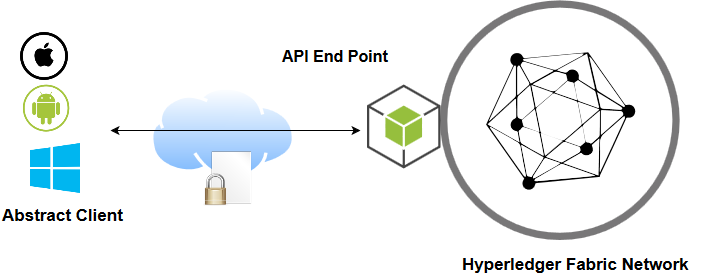
\includegraphics[width=10cm,height=8cm]{images/issues.png}
\caption{Obscuring the Network by Using the Node.js App }
\label{fig:issues}
\end{figure}

\section{Future Work} 

Based on our reusable and modular design we could adopt any complex business logic by simply modifying the chaincode. Furthermore, we could introduce more roles such as, Researchers and verifiers who could have more privileges like banning other users who scam the platform and prevent any malicious behavior. 
 
